% ==============================================================
% Experiment 3: Basic RC Circuits - High-pass and Low-pass Filters
% Meant to be inserted via \input{expt3.tex} in the root document.
% Requires in the root preamble: circuitikz, amsmath, booktabs,
%                                 pgfplots, \usepgfplotslibrary{groupplots}
%                                 \pgfplotsset{compat=1.18}
% ==============================================================

\chapter{Experiment 3: Basic RC Circuits - High-pass and Low-pass Filters}

\section{Aim}
To design, construct and study the frequency response (Bode plot) and
time-domain behaviour of a first-order RC low-pass filter and a first-order
RC high-pass filter for a specified cutoff frequency.
\section{Pre-Lab Exercise}
Before performing the experiment, simulate the circuits and verify the designs using LTspice or any other circuit simulation software. 
\section{Apparatus / Components Required}
\begin{center}
	\begin{tabular}{@{}cll@{}}
		\toprule
		S.No. & Component & Specification \\
		\midrule
		1 & Resistor $R$ & As designed \\
		2 & Capacitor $C$ & As designed \\
		3 & Function Generator & Sine and square wave, up to $100\ \text{kHz}$ \\
		4 & Cathode Ray Oscilloscope (CRO) & Dual channel \\
		5 & Breadboard and connecting wires & -- \\
		\bottomrule
	\end{tabular}
\end{center}

\section{Theory}
\emph{We have seen the RC circuit in the pre-lab activity, where we used this circuit to familiarise the DSO and the funciton generator and the measurement techniques.}

A first-order RC low-pass filter (LPF) passes low frequencies and attenuates (reduces the amplitude of)
high frequencies, while a first-order RC high-pass filter (HPF) does the
opposite. Both are built from the same two components, only the position of
$R$ and $C$ is interchanged, and both share the same cutoff (or corner)
frequency
\[
f_c = \frac{1}{2\pi R C}.
\]
The attenuation/gain is measured in terms of the unit decibel (dB), where a dB is defined as follows:

\[
dB = 20\log_{10}\frac{V_{out}}{V_{in}}
\]
\paragraph{Low-pass filter.} With $R$ in series and $C$ shunting the output
to ground, the transfer function is
\[
H_{LP}(f) = \frac{V_{out}}{V_{in}} = \frac{1}{1 + j\,(f/f_c)}, \qquad
|H_{LP}(f)| = \frac{1}{\sqrt{1+(f/f_c)^2}}, \qquad
\angle H_{LP}(f) = -\tan^{-1}\!\left(\frac{f}{f_c}\right).
\]

\paragraph{High-pass filter.} With $C$ in series and $R$ shunting the output
to ground, the transfer function is
\[
H_{HP}(f) = \frac{V_{out}}{V_{in}} = \frac{j\,(f/f_c)}{1 + j\,(f/f_c)}, \qquad
|H_{HP}(f)| = \frac{f/f_c}{\sqrt{1+(f/f_c)^2}}, \qquad
\angle H_{HP}(f) = 90^\circ - \tan^{-1}\!\left(\frac{f}{f_c}\right).
\]

At $f = f_c$, both filters attenuate the signal to $1/\sqrt{2}$ ($-3\ \text{dB}$)
of the input, with a phase shift of $-45^\circ$ (LPF) or $+45^\circ$ (HPF).

\paragraph{Time-domain view.} When the input is a square wave:
\begin{itemize}
	\item If $RC \gg T$ (period), the LPF cannot follow the fast transitions and
	behaves like an \emph{integrator}, producing a triangular/rounded output.
	\item If $RC \ll T$, the HPF passes only the transitions and behaves like a
	\emph{differentiator}, producing narrow decaying spikes at each edge.
\end{itemize}

\section{Design}

\paragraph{Specifications.}
\[
f_c = 1\ \text{kHz}
\]

\paragraph{Step 1: Choose a standard capacitor value.}
\[
C = 0.1\ \mu\text{F} \quad (\text{standard value})
\]

\paragraph{Step 2: Compute $R$ for the required cutoff frequency.}
\[
R = \frac{1}{2\pi f_c C} = \frac{1}{2\pi \times 1000 \times 0.1\times10^{-6}}
\approx 1591.5\ \Omega
\]
Nearest standard value: $\boxed{R = 1.5\ \text{k}\Omega}$.

\paragraph{Step 3: Verify actual cutoff frequency.}
\[
f_c = \frac{1}{2\pi R C} = \frac{1}{2\pi \times 1500 \times 0.1\times10^{-6}}
\approx 1.061\times 10^{3}\ \text{Hz} \approx 1\ \text{kHz} \quad \text{(OK)}
\]

\paragraph{Final design summary (common to both filters).}
\begin{center}
	\begin{tabular}{@{}ll@{}}
		\toprule
		Parameter & Value \\
		\midrule
		Resistor $R$ & $1.5\ \text{k}\Omega$ \\
		Capacitor $C$ & $0.1\ \mu\text{F}$ \\
		Cutoff frequency $f_c$ & $\approx 1\ \text{kHz}$ \\
		Attenuation at $f_c$ & $-3\ \text{dB}$ ($0.707\times V_{in}$) \\
		Phase shift at $f_c$ & $-45^\circ$ (LPF), $+45^\circ$ (HPF) \\
		\bottomrule
	\end{tabular}
\end{center}

\section{Circuit Diagrams}
The circuits of the RC low-pass and high-pass filters are shown in Fig.~\ref{fig:rc-lpf} and Fig.~\ref{fig:rc-hpf} respectively. 

\begin{figure}[htbp]
	\centering
	\begin{circuitikz}[american, scale=1.05, line width=0.8pt]
		\draw
		(0,0) to[sinusoidal voltage source, l=$v_{in}(t)$] (0,3)
		(0,3) to[R, l=$R$, *-*] (3,3)
		(3,3) to[C, l=$C$, -*] (3,0)
		(3,0) to[short] (0,0)
		;
		\draw (3,3) node[right]{$v_{out}(t)$};
		\draw (0,0) node[ground]{};
	\end{circuitikz}
	\caption{First-order RC low-pass filter}
	\label{fig:rc-lpf}
\end{figure}

\begin{figure}[!ht]
	\centering
	\begin{circuitikz}[american, scale=1.05, line width=0.8pt]
		\draw
		(0,0) to[sinusoidal voltage source, l=$v_{in}(t)$] (0,3)
		(0,3) to[C, l=$C$, *-*] (3,3)
		(3,3) to[R, l=$R$, -*] (3,0)
		(3,0) to[short] (0,0)
		;
		\draw (3,3) node[right]{$v_{out}(t)$};
		\draw (0,0) node[ground]{};
	\end{circuitikz}
	\caption{First-order RC high-pass filter}
	\label{fig:rc-hpf}
\end{figure}

\section{Procedure}

\paragraph{(a) Frequency response (Bode plot).}
\begin{enumerate}
	\item Connect the circuit as shown in Figure~\ref{fig:rc-lpf} (repeat later for Figure~\ref{fig:rc-hpf}).
	\item Apply a sine wave of constant amplitude $V_{in}$ from the function generator.
	\item Vary the frequency from about $10\ \text{Hz}$ to $100\ \text{kHz}$ in suitable steps (more closely spaced near $f_c$).
	\item At each frequency, measure $V_{out}$ and the phase difference between $v_{in}(t)$ and $v_{out}(t)$ using the CRO (dual trace / Lissajous method). 
	\item Compute gain in dB as $20\log_{10}(V_{out}/V_{in})$. Tabulate the observations/calculations as in Table~\ref{tab:obsFreqResp}.
	\item Plot gain (dB) and phase (degrees) versus frequency (log scale) --- the Bode magnitude and phase plots. Use a semi-log graph-sheet for plotting the frequency response.
	\item Gain (dB) versus frequency for the LPF and HPF, each expected to approach the shapes shown in Figures~\ref{fig:bode-lpf} and~\ref{fig:bode-hpf}, 		with a $-3\ \text{dB}$ point at $f_c$ and asymptotic slopes of $\pm 20\ \text{dB/decade}$ away from $f_c$.
	\item Phase (degrees) versus frequency for the LPF and HPF, passing through $-45^\circ$ and $+45^\circ$ respectively at $f_c$.
\end{enumerate}

\paragraph{(b) Time-domain response.}
\begin{enumerate}
	\item Apply a square wave at a frequency well below $f_c$ (for the LPF, to observe near-integrator behaviour) and well above $f_c$ (for the HPF, to observe near-differentiator behaviour).
	\item Observe and sketch $v_{in}(t)$ and $v_{out}(t)$ simultaneously on the CRO.
	\item Compare the observed waveforms with Figures~\ref{fig:waveform-lpf} and~\ref{fig:waveform-hpf}.
\end{enumerate}

\section{Tabulation}

\paragraph{Low-pass filter.}
\begin{center}
	\begin{tabular}{@{}cccc@{}}
		\toprule
		Frequency (Hz) & $V_{out}$ (V) & Gain $= 20\log_{10}(V_{out}/V_{in})$ (dB) & Phase (deg) \\
		\midrule
		10    & & & \\
		100   & & & \\
		500   & & & \\
		1000  & & & \\
		2000  & & & \\
		5000  & & & \\
		10000 & & & \\
		50000 & & & \\
		\bottomrule
	\end{tabular}
\end{center}

\paragraph{High-pass filter.}
\begin{center}
	\begin{tabular}{@{}cccc@{}}
		\toprule
		Frequency (Hz) & $V_{out}$ (V) & Gain $= 20\log_{10}(V_{out}/V_{in})$ (dB) & Phase (deg) \\
		\midrule
		10    & & & \\
		100   & & & \\
		500   & & & \\
		1000  & & & \\
		2000  & & & \\
		5000  & & & \\
		10000 & & & \\
		50000 & & & \\
		\bottomrule
	\end{tabular}
\end{center}
\subsection*{Bode Diagrams}
The frequency-response curves (gain and phase Vs frequency) are known as Bode diagrams (afer the inventor Hendrik Wade Bode). The y-axis of the gain plot uses the dB unit, and the phase plot uses the phase lag/lead in degrees. The x-axis is in log-scale, and frequencies in decades are marked. The sample Bode diagrams are as shown in Figs.~\ref{fig:bode-lpf} and \ref{fig:bode-hpf}. 
\begin{figure}[ht!]
	\centering
	\begin{tikzpicture}
		\begin{groupplot}[
			group style={group size=1 by 2, vertical sep=1.7cm},
			width=10cm, height=4.2cm,
			xmode=log,
			xmin=10, xmax=100000,
			xlabel={Frequency (Hz)},
			grid=major,
			domain=10:100000,
			samples=300,
			]
			\nextgroupplot[
			ylabel={Gain (dB)},
			ymin=-40, ymax=5,
			title={Low-pass filter -- magnitude response},
			]
			\addplot[thick, blue] {-10*log10(1+(x/1000)^2)};
			\draw[dashed, gray] (axis cs:1000,-40) -- (axis cs:1000,5);
			\node[gray, above] at (axis cs:1000,-3) {\footnotesize $f_c$};
			\nextgroupplot[
			ylabel={Phase (deg)},
			ymin=-100, ymax=10,
			ytick={0,-45,-90},
			title={Low-pass filter -- phase response},
			]
			\addplot[thick, red] {-atan(x/1000)};
			\draw[dashed, gray] (axis cs:1000,-100) -- (axis cs:1000,10);
		\end{groupplot}
	\end{tikzpicture}
	\caption{Bode plot of the RC low-pass filter ($f_c \approx 1\ \text{kHz}$)}
	\label{fig:bode-lpf}
\end{figure}

\begin{figure}[ht!]
	\centering
	\begin{tikzpicture}
		\begin{groupplot}[
			group style={group size=1 by 2, vertical sep=1.7cm},
			width=10cm, height=4.2cm,
			xmode=log,
			xmin=10, xmax=100000,
			xlabel={Frequency (Hz)},
			grid=major,
			domain=10:100000,
			samples=300,
			]
			\nextgroupplot[
			ylabel={Gain (dB)},
			ymin=-40, ymax=5,
			title={High-pass filter -- magnitude response},
			]
			\addplot[thick, blue] {20*log10(x/1000)-10*log10(1+(x/1000)^2)};
			\draw[dashed, gray] (axis cs:1000,-40) -- (axis cs:1000,5);
			\node[gray, above] at (axis cs:1000,-3) {\footnotesize $f_c$};
			\nextgroupplot[
			ylabel={Phase (deg)},
			ymin=-10, ymax=100,
			ytick={0,45,90},
			title={High-pass filter -- phase response},
			]
			\addplot[thick, red] {90-atan(x/1000)};
			\draw[dashed, gray] (axis cs:1000,-10) -- (axis cs:1000,100);
		\end{groupplot}
	\end{tikzpicture}
	\caption{Bode plot of the RC high-pass filter ($f_c \approx 1\ \text{kHz}$)}
	\label{fig:bode-hpf}
\end{figure}

\section{Sample Waveforms (Square Wave Input)}
The time-domain behaviour of the RC circuit can be understood by studying the response to a square-wave of variable frequency, the waveforms of which are shown in Figs.~\ref{fig:waveform-lpf} and \ref{fig:waveform-hpf}. It can be seen that for $RC\gg T/2$, the RC low-pass filter circuit acts as an integrator, whereas for the RC high-pass circuit (with C and R interchanged), behaves as a differentiator when $RC \ll T/2$. Further, note that the waveform given in Fig.~\ref{fig:waveform-hpf} are obtained under the constraint that $R\gg R_{out}$ of the source (function generator).

\begin{figure}[ht!]
	\centering
	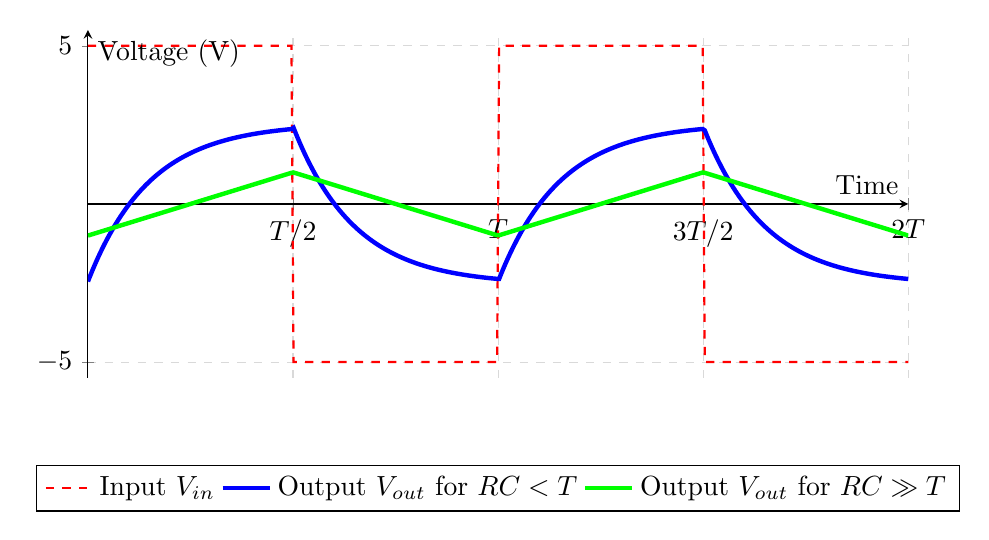
\begin{tikzpicture}
		\begin{axis}[
			width=12cm, height=6cm,
			axis lines=middle,
			xlabel={Time},
			ylabel={Voltage (V)},
			xmin=0, xmax=20,
			xtick={0,5,10,15,20}, xticklabels={$0$,$T/2$,$T$,$3T/2$,$2T$},
			ymin=-5.5, ymax=5.5,
			grid=major,
			grid style={dashed, gray!30},
			legend style={at={(0.5,-0.25)}, anchor=north, legend columns=-1},
			domain=0:20,
			samples=400
			]
			% 1. Input: 0V to 5V Square Wave (Period = 10ms, Duty Cycle = 50%)
			\addplot[red, thick, dashed, samples y=0] 
			{mod(x, 10) < 5 ? 5 : -5};
			\addlegendentry{Input $V_{in}$}
			
			% 2. Output: Exact Steady-State Piece-wise Exponential Response (tau = 1.5ms)
			% V_min ≈ 0.94V and V_max ≈ 4.06V are the calculated steady-state limits.
			\addplot[blue, ultra thick, no marks] {
				mod(x, 10) < 5 ? 
				(5 * (1-exp(-mod(x, 5) / 1.5)))-2.45 : % Charging phase (HIGH)
				(2.45-5*(1-exp(-mod(x, 5) / 1.5)))            % Discharging phase (LOW)
			};
			\addlegendentry{Output $V_{out}$ for $RC < T$}
			%modify following to triangular
			\addplot[green, ultra thick, no marks] {
				mod(x, 10) < 5 ? 
				(-1+0.4*mod(x,5) : % Charging phase (HIGH)
				(1-0.4*mod(x,5))            % Discharging phase (LOW)
			};
			\addlegendentry{Output $V_{out}$ for $RC \gg T$}
		\end{axis}
	\end{tikzpicture}
	\caption{Low-pass filter response to a square wave (rounded/ramped output)}
	\label{fig:waveform-lpf}
\end{figure}

\begin{figure}[ht!]
	\centering
	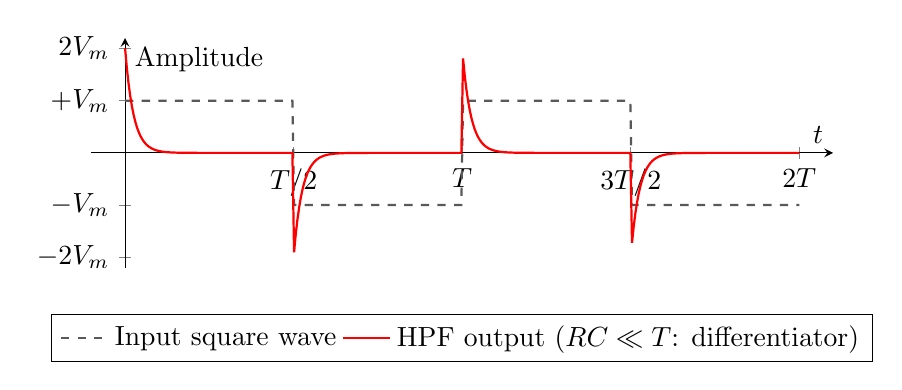
\begin{tikzpicture}
		\begin{axis}[
			width=11cm, height=4.5cm,
			axis lines=middle,
			xlabel={$t$}, ylabel={Amplitude},
			legend style={
				at={(0.5,-0.2)}, 
				anchor=north,
				legend columns=-1, % -1 arranges all entries in a single row
			},
			% Ensures the nodes align correctly
			legend cell align=left,
			xmin=-0.2, xmax=4.2, ymin=-2.2, ymax=2.2,
			xtick={0,1,2,3,4}, xticklabels={$0$,$T/2$,$T$,$3T/2$,$2T$},
			ytick={2,1,-1,-2}, yticklabels={$2V_m$, $+V_m$,$-V_m$, $-2V_m$},
			domain=0:4, samples=400, clip=false,
			]
			\addplot[thick, dashed, gray!70!black]
			{ifthenelse(mod(x,2)<1, 1, -1)};
			\addplot[thick, red]
			{ifthenelse(mod(x,2)<1,
				2*exp(-mod(x,2)/0.05),
				-2*exp(-(mod(x,2)-1)/0.05))};
			\legend{Input square wave, HPF output ($RC \ll T$: differentiator)}
		\end{axis}
	\end{tikzpicture}
	\caption{High-pass filter response to a square wave (decaying spikes at transitions)}
	\label{fig:waveform-hpf}
\end{figure}

\section{Result}
First-order RC low-pass and high-pass filters were designed for a cutoff
frequency of $1\ \text{kHz}$ using $R = 1.5\ \text{k}\Omega$ and
$C = 0.1\ \mu\text{F}$. Their frequency response (Bode plots) and time-domain
behaviour with a square-wave input were studied and verified experimentally
against the theoretical response.
\begin{explorebox}
	The output impedance of the source (function generator) has an impact on practical measurements. Hence, while checking the output waveforms of the high-pass (or differentiator) circuit, the resistance value should be much higher than that of the output impedance of the function generator (typically, $50\ \Omega$). For satisfying the condition $RC \ll T/2$, we may choose a higher R and a lower C, or vice-versa. Try with both designs and see how the waveforms differ in each case practically, and explain why. What is the effect in the case of the integrator? When simulating, you may experiment with/without a source resistance to see the effects.
\end{explorebox}

\section{Questions}
\begin{enumerate}
	\item Derive the transfer function of a first-order RC low-pass filter.
	\item Why do the LPF and HPF built from the same $R$ and $C$ have the same
	cutoff frequency?
	\item What is the significance of the $-3\ \text{dB}$ point?
	\item What is the asymptotic roll-off rate of a first-order filter, in
	dB/decade?
	\item Under what condition does an RC low-pass filter behave as an
	integrator, and a high-pass filter as a differentiator?
	\item Why is the RC circuit (both LPF and HPF) in this experiment called  ``first-order'' filters?
	\item How would you extend this circuit to a second-order filter, and
	what advantage would that give?
	\item What are the effects of function generator output impedance on the design/expected waveforms of the RC circuit?
	\item How do the integrator and differentiator circuits behave when the input signal has a DC added to it ($\pm V_{dc}$)?
\end{enumerate}